% Benchmark B: two equal cylinders, all-pairs Gauss-point contact,
% comparison against the Hertz line-contact solution
\documentclass[border=8pt]{standalone}
\usepackage{tikz}
\usetikzlibrary{arrows.meta,patterns.meta}

\newcommand{\rollersym}[3]{%
  \begin{scope}[shift={(#1,#2)}, rotate=#3]
    \draw[fill=white] (0,0) -- (-0.09,0.16) -- (0.09,0.16) -- cycle;
    \draw[fill=white] (-0.075,0.20) circle (0.022);
    \draw[fill=white] (0.075,0.20) circle (0.022);
    \draw (-0.11,0.235) -- (0.11,0.235);
    \draw[gray] (-0.13,0.245) -- (-0.10,0.285);
    \draw[gray] (-0.06,0.245) -- (-0.03,0.285);
    \draw[gray] (0.01,0.245) -- (0.04,0.285);
    \draw[gray] (0.08,0.245) -- (0.11,0.285);
  \end{scope}
}

\begin{document}
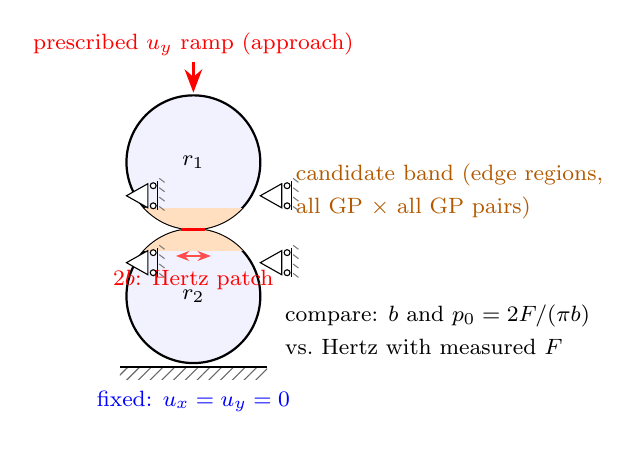
\begin{tikzpicture}[>={Stealth}, scale=1.7]

  % ---- two equal disks (r = 0.5), tangent at (0,0.5) ----
  \draw[thick, fill=blue!5] (0,1.0) circle (0.5);   % disk 1 (upper)
  \draw[thick, fill=blue!5] (0,0.0) circle (0.5);   % disk 2 (lower)
  \node at (0.0, 1.0) {\footnotesize $r_1$};
  \node at (0.0, 0.0) {\footnotesize $r_2$};

  % ---- candidate band on both arcs (all-pairs pairing zone) ----
  \begin{scope}
    \clip (0,1.0) circle (0.5);
    \fill[orange!25] (-0.6, 0.5) rectangle (0.6, 0.66);
  \end{scope}
  \begin{scope}
    \clip (0,0.0) circle (0.5);
    \fill[orange!25] (-0.6, 0.34) rectangle (0.6, 0.5);
  \end{scope}
  \node[right, orange!70!black, inner sep=2pt, align=left] at (0.72, 0.78)
    {\footnotesize candidate band (edge regions,\\
     \footnotesize all GP $\times$ all GP pairs)};

  % ---- Hertz patch ----
  \draw[red, very thick] (-0.09, 0.5) -- (0.09, 0.5);
  \draw[{Stealth}-{Stealth}, red!70] (-0.13, 0.30) -- (0.13, 0.30);
  \node[below, red, inner sep=2pt] at (0.0, 0.24) {\footnotesize $2b$: Hertz patch};

  % ---- prescribed u_y on top ----
  \draw[red, very thick, ->] (0, 1.75) -- (0, 1.52);
  \node[above, red, inner sep=2pt] at (0, 1.75)
    {\footnotesize prescribed $u_y$ ramp (approach)};

  % ---- fixed ground below ----
  \fill[pattern={Lines[angle=45, distance=3pt]}, pattern color=black!60]
    (-0.55, -0.62) rectangle (0.55, -0.53);
  \draw[thick] (-0.55, -0.53) -- (0.55, -0.53);
  \node[below, blue, inner sep=3pt] at (0.0, -0.64)
    {\footnotesize fixed: $u_x = u_y = 0$};

  % ---- side rollers ----
  \rollersym{-0.5}{0.75}{-90}
  \rollersym{0.5}{0.75}{-90}
  \rollersym{-0.5}{0.25}{-90}
  \rollersym{0.5}{0.25}{-90}

  % ---- comparison quantities ----
  \node[right, inner sep=3pt, align=left] at (0.62, -0.25)
    {\footnotesize compare: $b$ and $p_0 = 2F/(\pi b)$\\
     \footnotesize vs.\ Hertz with measured $F$};

\end{tikzpicture}
\end{document}
